\newpage
\section{Frequency domain editor}
Related YouTube videos:
\begin{figure}[H]

\begin{tabular}{ c l }


\includegraphics[width=0.05\textwidth]{./images/youtube.png}

&
\href{https://www.youtube.com/watch?v=NJAsZeiB5FU}{Simulating impedance spectroscopy (IS) in solar cells.}

\end{tabular}
\end{figure}

\subsection{Overview}
The frequency plugin allows you to simulate the frequency domain response of the device.  Using this tool one can perform impedance spectroscopy, as well as optically excited measurements such as Intensity Modulated Photo Spectroscopy (IMPS), Intensity Modulated Voltage Spectroscopy (IMVS). The  domain editor allows you to configure frequency domain simulations. This is shown below in Figures \ref{fig:fx_domain_mesh} and \ref{fig:fx_domain_circuit}. On the left hand side is the frequency domain mesh editor this is used to define which frequencies will be simulated.  Figure \ref{fig:fx_domain_circuit} shows the \emph{circuit} tab of the frequency domain window, this sets the electrical configuration of the simulation. One can either simulate an ideal diode (this is the fastest type of simulation to perform), a diode with parasitic components or a diode in open circuit. An ideal diode would be used for IMPS simulations while the open circuit model would be used for IMVS simulations. Pick the circuit depending on what conditions you want to simulate. If you want examples of frequency domain simulation look in the new simulation window under Organic Solar cells, some of the PM6:Y6 devices have examples of frequency domain simulations already set up.
\\
\\
\noindent
\begin{minipage}{0.5\textwidth}
	\centering
	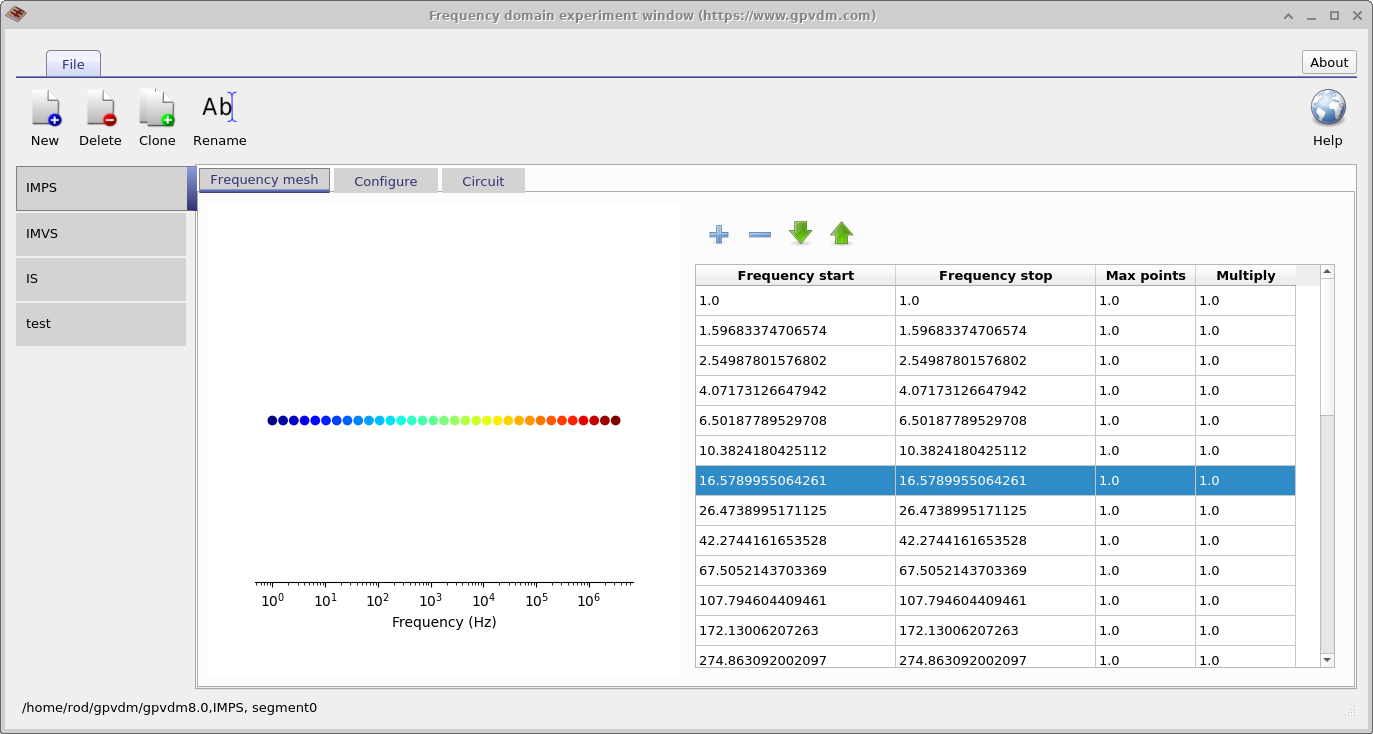
\includegraphics[width=\linewidth,height=0.8\linewidth]{./images/sim_editors/fx_domain_editor.png}
	\captionof{figure}{The frequency domain editor window}
	\label{fig:fx_domain_mesh}
\end{minipage}
\hspace{4pt}
\begin{minipage}[]{0.5\linewidth}
	\centering
	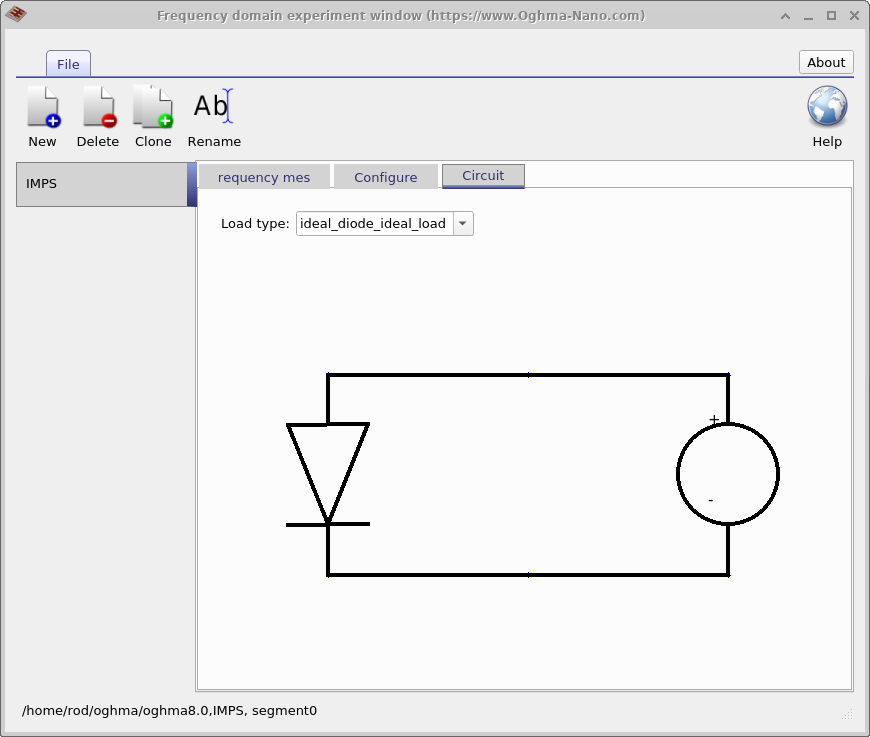
\includegraphics[width=\linewidth,height=0.8\linewidth]{./images/sim_editors/fx_domain_circuit.png}
	\captionof{figure}{A circuit set up for frequency domain simulations.}
	\label{fig:fx_domain_circuit}
\end{minipage}

\subsubsection{Large signal or small signal}
There are two ways to simulate frequency domain simulations in a device model, a large signal approach or a small signal approach. The small signal approach assumes the problem we are looking at varies linearly around a DC point, this may or may not be true depending on the conditions one is looking at. This method is however computationally fast.  The second approach is to use a large signal approach and rather than simulating linear variation around a set point one simulates the time domain response of the device in full for each wavelength of interest.  This method is cope better non-linear systems and one does not need to worry if one is in the large or small signal regime but is slower.  OghmaNano uses the large signal approach.

\subsection{Inputs}
In Figure \ref{fig:fx_domain_option} the \emph{Configure} tab of the frequency domain window can be seen. This decides exactly how the simulation will perform. These are described below in table \ref{tab:fx_inputs}

\begin{table}
\begin{center}
\begin{tabular}{ |l|p{8cm}| } 
 \hline
	File name 					& 	Description  \\ 
 \hline
	$V_{external}$				&	The external voltage applied to the cell\\ 
	Simulation type				&	Leave this as Large signal.\\
	Load resistor				&	External load resistor, this should be usually set to zero.\\ 
	FX domain mesh points 		&	The number of time steps used to simulate each cycle\\ 
	Cycles to simulate 			&	The number of complete periods of any given frequency that are simulated \\ 
	Excite with					&	How the device is excited, either optically or electrically.\\ 
	Measure 					&	What is measured, current or voltage.\\
	Modulation depth			&	How deep is the DC voltage/current modulated\\
 	Periods to fit				&	The number of frequency domain cycles that are fit to extract phase angle\\
 	Output verbosity to disk	&	How much data is dumped to disk (described in other sections)\\
 	Output verbosity to screen	&	How much data is shown on the creen (described in other sections)\\
 \hline
\end{tabular}
\caption{Files produced by the time domain simulation}
\label{tab:fx_inputs}
\end{center}
\end{table}

\begin{figure}
\centering
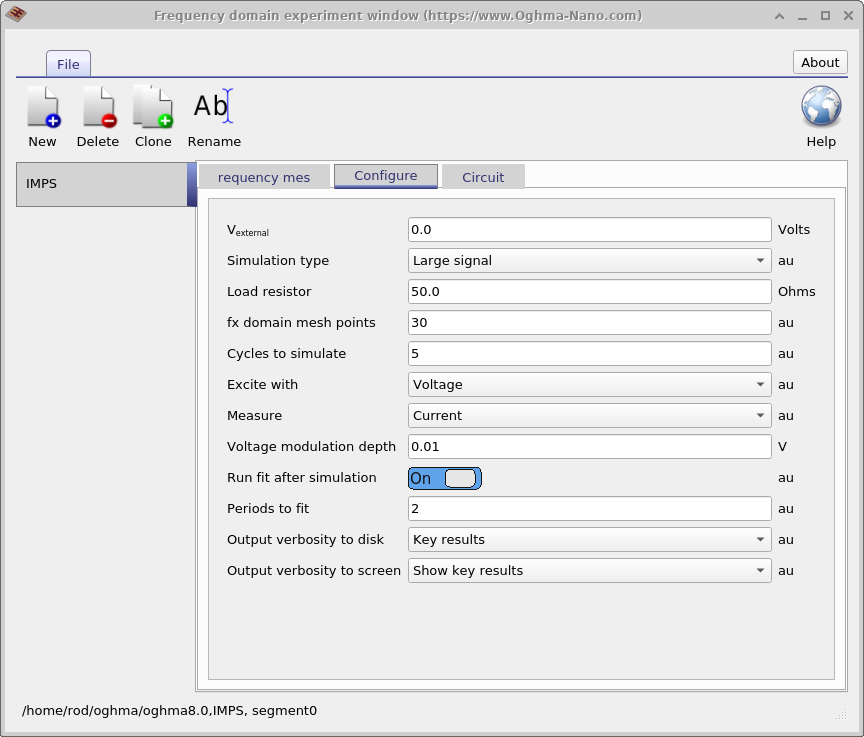
\includegraphics[width=0.7\linewidth,height=0.5\linewidth]{./images/sim_editors/fx_domain_options.png}
\caption{Configuring a frequency domain simulation}
\label{fig:fx_domain_option}
\end{figure}


\subsection{Outputs}


\begin{table}[H]
\begin{center}
\begin{tabular}{ |c|c|c| } 
 \hline
	File name 			& 	Description  \\ 
 \hline
	real\_imag.csv		&	Re(i(fx)) v.s. Im(i(fx))\\ 
	fx\_imag.csv		&	fx v.s. Im(i(fx))\\
	fx\_real.csv 		&	fx v.s. Re(i(fx))\\ 
	fx\_abs.csv 		&	fx v.s. $\lvert i(fx) \rvert$\\ 
	fx\_phi.csv 		&	fx v.s. $ \angle i(fx)$ \\ 
	fx\_C.csv 			&	fx v.s. Capacitance\\ 
	fx\_R.csv 			&	fx v.s. Resistance\\ 
 \hline
\end{tabular}
\caption{Files produced by the time domain simulation}
\label{tab:ce_output}
\end{center}
\end{table}

